%the development background of Qwen2.5-VL and highlights its latest advancements as a vision-language model, particularly focusing on breakthroughs in temporal and spatial awareness. It also outlines key features such as visual understanding, document parsing, video comprehension, object localization, and structured output generation.
Large vision-language models ( LVLMs )~\citep{gpt4o,sonnet3_5,team2023gemini,wang2024qwen2} represent a pivotal breakthrough in artificial intelligence, signaling a transformative approach to multimodal understanding and interaction. By seamlessly integrating visual perception with natural language processing, these advanced models are fundamentally reshaping how machines interpret and analyze complex information across diverse domains. Despite significant advancements in multimodal large language models, the current capabilities of these models can be likened to the middle layer of a sandwich cookie—competent across various tasks but falling short of exceptional performance. Fine-grained visual tasks form the foundational layer of this analogy. In this iteration of Qwen2.5-VL, we are committed to exploring fine-grained perception capabilities, aiming to establish a robust foundation for LVLMs and create an agentic amplifier for real-world applications. The top layer of this framework is multi-modal reasoning, which is enhanced by leveraging the latest Qwen2.5 LLM and employing multi-modal QA data construction.

% related work 
A spectrum of works have promoted the development of multimodal large models, characterized by architectural design, visual input processing, and data curation. One of the primary drivers of progress in LVLMs is the continuous innovation in architecture. The studies presented in~\citep{flamingo, blip, blip2, llava, llava1.5, wang2024emu3, zhang2024internlm,wang2023internimage} have incrementally shaped the current paradigm, which typically consists of a visual encoder, a cross-modal projector, and LLM. Fine-grained perception models have emerged as another crucial area. Models like ~\citep{xiao2023florence,grounding_dino,ren2024grounding, ferretv2,zhang2024omg,kosmos2,deitke2024molmo} have pushed the boundaries of what is possible in terms of detailed visual understanding. The architectures of Omni~\citep{li2024baichuan,li2025baichuan,ye2024x} and MoE~\citep{riquelme2021scaling,lee2024moai,li2024uni,li2024aria,wu2024deepseek} also inspire the future evolution of LVLMs. Enhancements in visual encoders~\citep{internvl, liu2024points,liang2025global} and resolution scaling~\citep{monkey,mplug-owl2,Otterhd} have played a pivotal role in improving the quality of practical visual understanding. Curating data with more diverse scenarios and higher-quality is an essential step in training advanced LVLMs. The efforts proposed in~\citep{guo2024mammoth,chen2024expanding, liu2024mminstruct, chen2024allava, tong2024cambrian, li2024llava} are highly valuable contributions to this endeavor. 

% the limitations of Current LVLMs
However, despite their remarkable progress, vision-language models currently face developmental bottlenecks, including computational complexity,  limited contextual understanding, poor fine-grained visual perception, and inconsistent performance across varied sequence length.

% \begin{figure*}[t]
% \centering
% 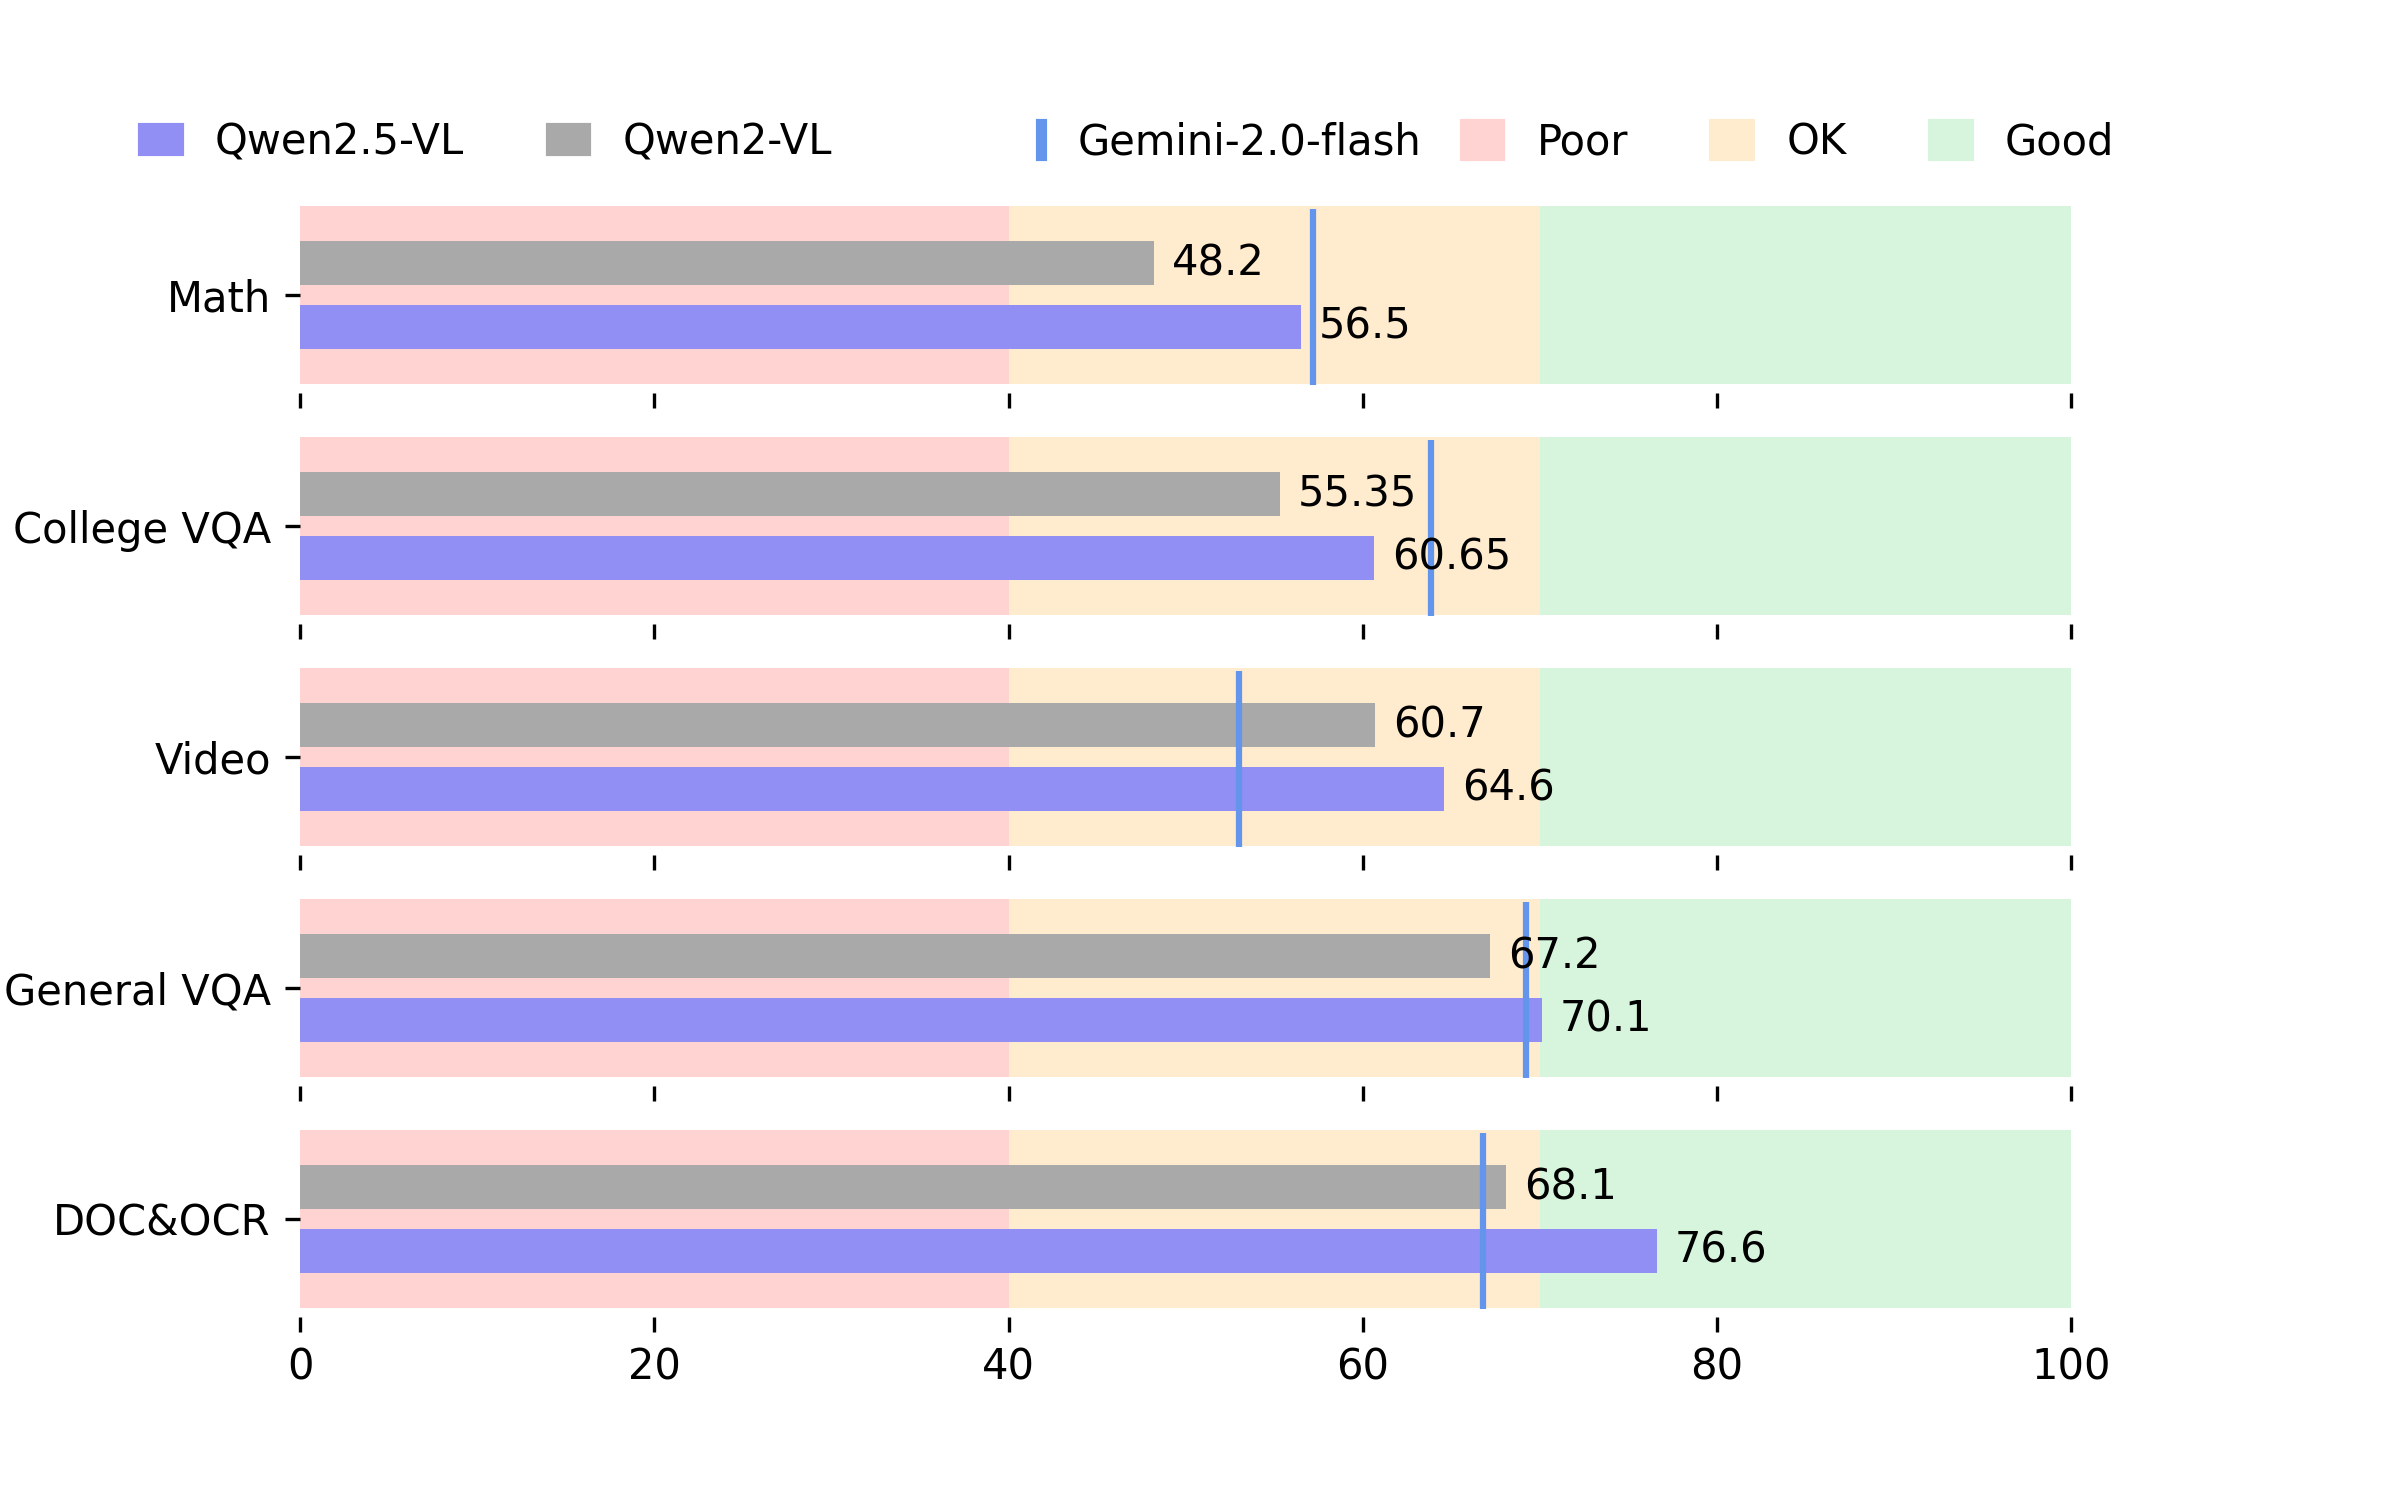
\includegraphics[width= 1\linewidth]{figures/bullet_introduction.png}
% \vspace{-10mm}
% \caption{Bullet Chart Comparison of the Qwen Series Models with Reference to Closed SOTA. Math ( MathVsita, MATH-Vsision ), College VQA ( MMMU, MMMU-PRO), Video ( Video-MME,MVBench, MMBench-Video, LVBench ), General VQA ( MMBench1.1, MegaBench, MMStar ), DOC\&OCR ( OCRBenchV1, OCRBenchV2, CC-OCR ). }
% \label{fig:intro}
% \end{figure*}
%the introduction of Qwen-vl
In this report, we introduce the latest work Qwen2.5-VL, which continues the open-source philosophy of the Qwen series, achieving and even surpassing top-tier closed-source models on various benchmarks. Technically, our contributions are four-folds: (1) We implement window attention in the visual encoder to optimize inference efficiency; (2) We introduce dynamic FPS sampling, extending dynamic resolution to the temporal dimension and enabling comprehensive video understanding across varied sampling rates; (3) We upgrade MRoPE in the temporal domain by aligning to absolute time, thereby facilitating more sophisticated temporal sequence learning; (4) We make significant efforts in curating high-quality data for both pre-training and supervised fine-tuning, further scaling the pre-training corpus from 1.2 trillion tokens to 4.1 trillion tokens.

%features
The sparkling characteristics of Qwen2.5-VL are as follows:
\begin{itemize}

 \item \textbf{Powerful document parsing capabilities:} Qwen2.5-VL upgrades text recognition to omni-document parsing, excelling in processing multi-scene, multilingual, and various built-in (handwriting, tables, charts, chemical formulas, and music sheets) documents.
 
 \item \textbf{Precise object grounding across formats:} Qwen2.5-VL unlocks improved accuracy in detecting, pointing, and counting objects, accommodating absolute coordinate and JSON formats for advanced spatial reasoning.
 
 \item \textbf{Ultra-long video understanding and fine-grained video grounding:} Our model extends native dynamic resolution to the temporal dimension, enhancing the ability to understand videos lasting hours while extracting event segments in seconds.
 
 \item \textbf{Enhanced agent Functionality for computer and mobile devices:} Leverage advanced grounding, reasoning, and decision-making abilities, boosting the model with superior agent functionality on smartphones and computers.
 
\end{itemize}